\documentclass{article} 

% include some useful things
\usepackage{verbatim}  % for printing unformatted text
\usepackage{graphicx}  % for including graphics, drawings, etc...
\usepackage{float}         % for controlling the location of figure and graphics on the page
\usepackage{amsmath}

%  Begin writing content below this line
\begin{document}

%  Print your name and the assignment number
\begin{center}{\huge  Rohan Chandra - hmwk9    Solutions}\end{center}

%%%%%%%%%%%%%%%%%%
%                Problem 1
%%%%%%%%%%%%%%%%%%
% \newpage
\section*{Question 2}
The residual curve for Logistic regression is below:


\begin{figure}[H]
\centering
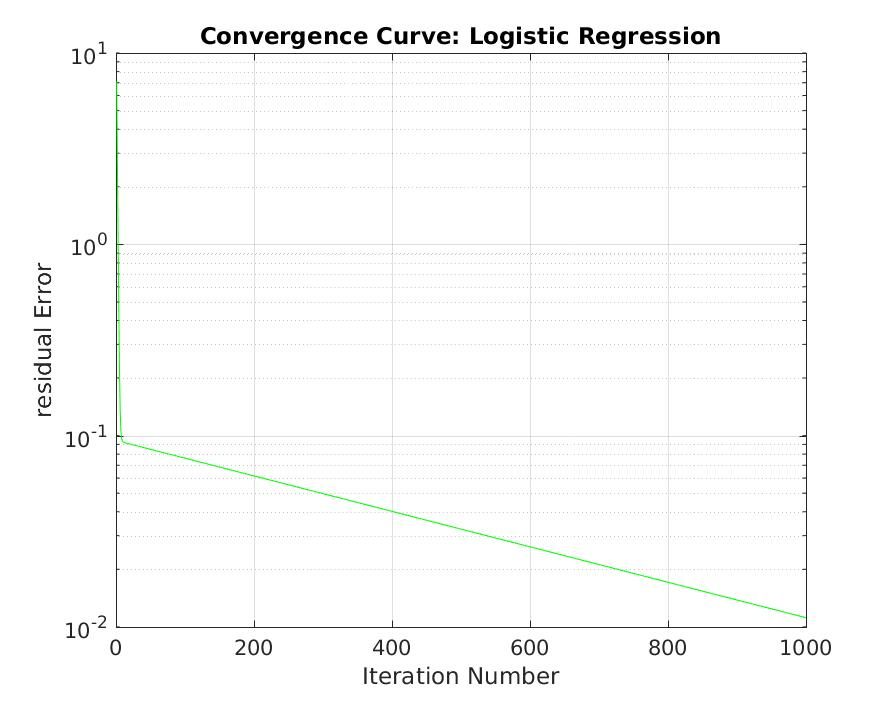
\includegraphics[width=1.2\linewidth]{LogisticRegression.jpg}
\caption{Logistic Regression convergence plot}
\end{figure}


\begin{figure}[H]
\centering
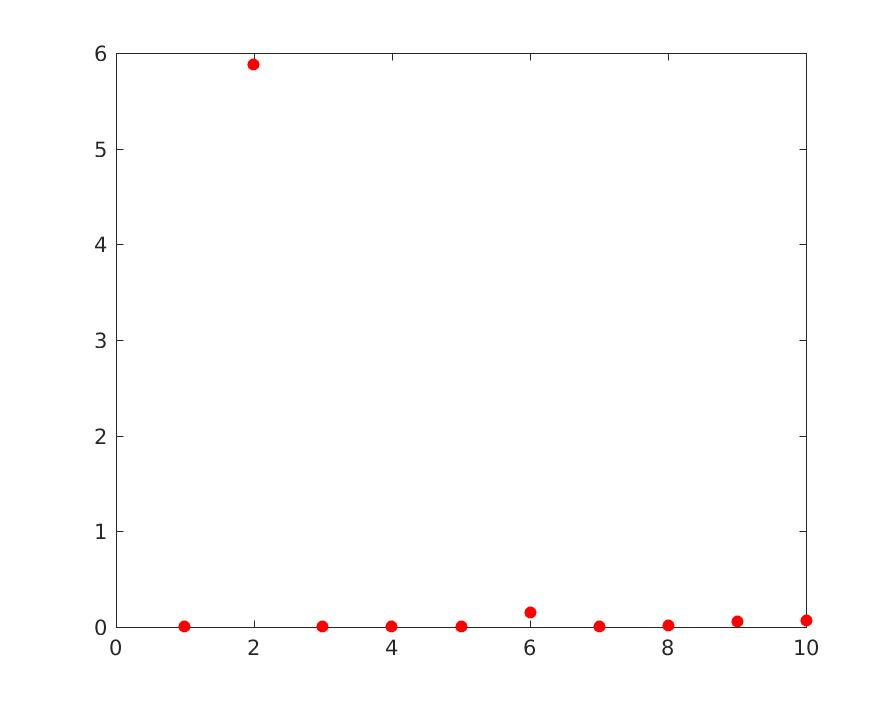
\includegraphics[width=1.2\linewidth]{LogisticRegression_plot.jpg}
\caption{Logistic Regression Solution plot}
\end{figure}




\section*{Question 3}

The residual curve for Total Variation is below:

\begin{figure}[H]
\centering
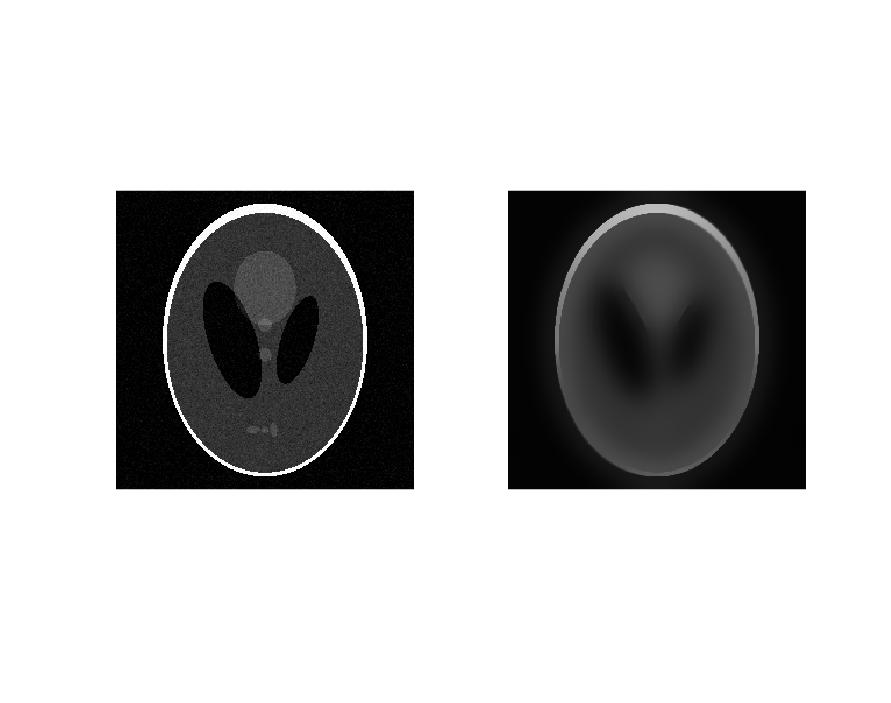
\includegraphics[width=1.2\linewidth]{TVplot.jpg}
\caption{Total Variation plot}
\end{figure}


\begin{figure}[H]
\centering
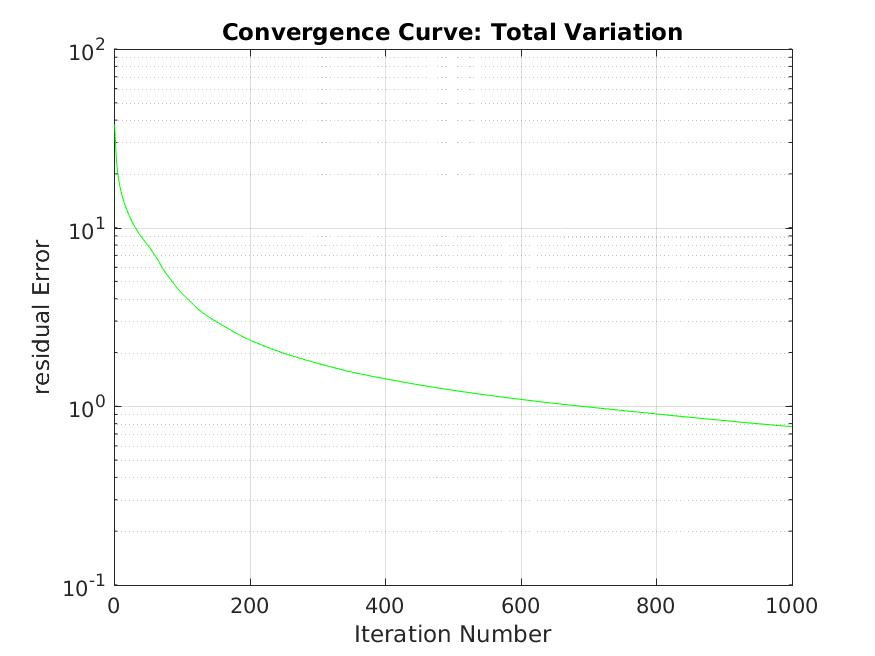
\includegraphics[width=1.2\linewidth]{TV_residual.jpg}
\caption{Total Variation convergence plot}
\end{figure}

\section*{Question 4}

The residual curve for Matrix Factorization is below:

\begin{figure}[H]
\centering
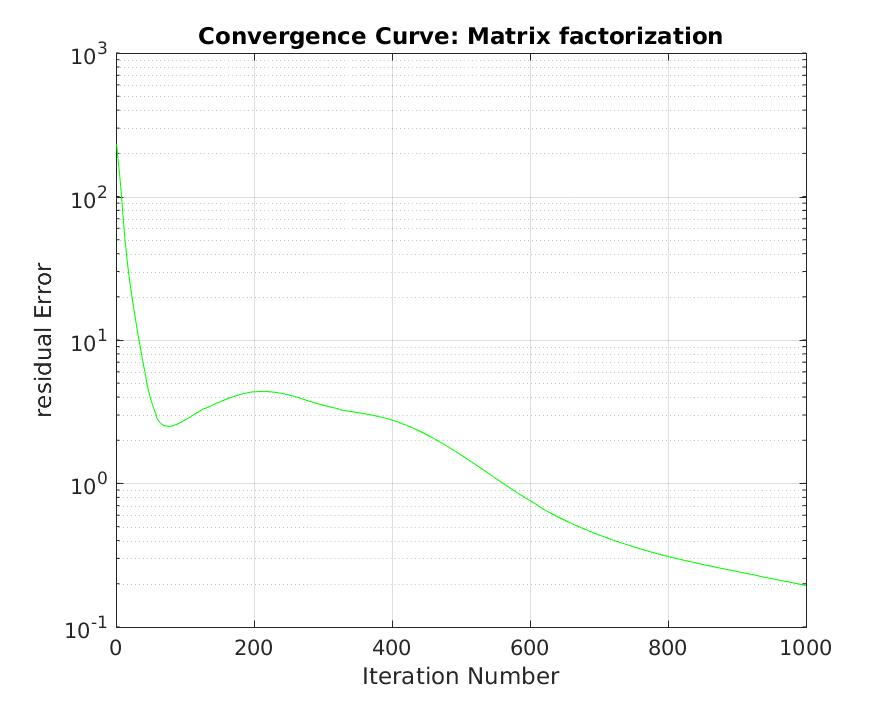
\includegraphics[width=1\linewidth]{MatrixFactorization_residual.jpg}
\caption{Matrix factorization convergence plot}
\end{figure}

Yes the recovery method works. Yes, it depends on how you initialize X and Y. It doesn't work if you inititalize both X and Y to zero.

\end{document}
